\documentclass[a4paper]{article}

\usepackage{inputenc}
\usepackage[british,UKenglish]{babel}
\usepackage{amsmath}
%\usepackage{titlesec}
\usepackage{color}
\usepackage{graphicx}
\usepackage{fancyref}
\usepackage{hyperref}
\usepackage{float}
\usepackage{scrextend}
\usepackage{setspace}
\usepackage{xargs}
\usepackage{multicol}
\usepackage{nameref}

\usepackage{mathrsfs}
\usepackage{sectsty}
\usepackage{multicol}
\usepackage{multirow}
\usepackage[procnames]{listings}
\usepackage{appendix}

\newcommand\tab[1][1cm]{\hspace*{#1}}
\hypersetup{colorlinks=true, linkcolor=black}
\interfootnotelinepenalty=10000

\newcommand{\cleancode}[1]{\begin{addmargin}[3em]{3em}\texttt{\textcolor{cleanOrange}{#1}}\end{addmargin}}
\newcommand{\cleanstyle}[1]{\text{\textcolor{cleanOrange}{\texttt{#1}}}}


\usepackage[colorinlistoftodos,prependcaption,textsize=footnotesize]{todonotes}
\newcommandx{\commred}[2][1=]{\textcolor{Red}
{\todo[linecolor=red,backgroundcolor=red!25,bordercolor=red,#1]{#2}}}
\newcommandx{\commblue}[2][1=]{\textcolor{Blue}
{\todo[linecolor=blue,backgroundcolor=blue!25,bordercolor=blue,#1]{#2}}}
\newcommandx{\commgreen}[2][1=]{\textcolor{OliveGreen}{\todo[linecolor=OliveGreen,backgroundcolor=OliveGreen!25,bordercolor=OliveGreen,#1]{#2}}}
\newcommandx{\commpurp}[2][1=]{\textcolor{Plum}{\todo[linecolor=Plum,backgroundcolor=Plum!25,bordercolor=Plum,#1]{#2}}}

\def\code#1{{\tt #1}}

\def\note#1{\noindent{\bf [Note: #1]}}

\makeatletter
%% The "\@seccntformat" command is an auxiliary command
%% (see pp. 26f. of 'The LaTeX Companion,' 2nd. ed.)
\def\@seccntformat#1{\@ifundefined{#1@cntformat}%
   {\csname the#1\endcsname\quad}  % default
   {\csname #1@cntformat\endcsname}% enable individual control
}
\let\oldappendix\appendix %% save current definition of \appendix
\renewcommand\appendix{%
    \oldappendix
    \newcommand{\section@cntformat}{\appendixname~\thesection\quad}
}
\makeatother


% "define" Scala
\usepackage[T1]{fontenc}  
\usepackage[scaled=0.82]{beramono}  
\usepackage{microtype} 

\sbox0{\small\ttfamily A}
\edef\mybasewidth{\the\wd0 }

\lstdefinelanguage{scala}{
  morekeywords={abstract,case,catch,class,def,%
    do,else,extends,false,final,finally,%
    for,if,implicit,import,match,mixin,%
    new,null,object,override,package,%
    private,protected,requires,return,sealed,%
    super,this,throw,trait,true,try,%
    type,val,var,while,with,yield},
  sensitive=true,
  morecomment=[l]{//},
  morecomment=[n]{/*}{*/},
  morestring=[b]",
  morestring=[b]',
  morestring=[b]"""
}

\usepackage{color}
\definecolor{dkgreen}{rgb}{0,0.6,0}
\definecolor{gray}{rgb}{0.5,0.5,0.5}
\definecolor{mauve}{rgb}{0.58,0,0.82}

% Default settings for code listings
\lstset{frame=tb,
  language=scala,
  aboveskip=3mm,
  belowskip=3mm,
  showstringspaces=false,
  columns=fixed, % basewidth=\mybasewidth,
  basicstyle={\small\ttfamily},
  numbers=none,
  numberstyle=\footnotesize\color{gray},
  % identifierstyle=\color{red},
  keywordstyle=\color{blue},
  commentstyle=\color{dkgreen},
  stringstyle=\color{mauve},
  frame=single,
  breaklines=true,
  breakatwhitespace=true,
  procnamekeys={def, val, var, class, trait, object, extends},
  procnamestyle=\ttfamily\color{red},
  tabsize=2
}

\lstnewenvironment{scala}[1][]
{\lstset{language=scala,#1}}
{}
\lstnewenvironment{cpp}[1][]
{\lstset{language=C++,#1}}
{}
\lstnewenvironment{bash}[1][]
{\lstset{language=bash,#1}}
{}
\lstnewenvironment{verilog}[1][]
{\lstset{language=verilog,#1}}
{}



\lstset{frame=, basicstyle={\footnotesize\ttfamily}}



\graphicspath{ {images/} }
\usepackage{ctex}

\begin{document}
\renewcommand{\contentsname}{目\ 录}
\renewcommand{\appendixname}{附录}
\renewcommand{\appendixpagename}{附录}
\renewcommand{\refname}{参考文献}
\renewcommand{\figurename}{图}
\renewcommand{\tablename}{表}
\renewcommand{\today}{\number\year 年 \number\month 月 \number\day 日}


\title{{\Huge MCP机理研究记录{\large\linebreak\\}}{\linebreak\linebreak}}
%please write your name, Student #, and Class # in Authors, student ID, and class # respectively
\author{翁俊$\  $张爱强$\  $续本达
}
\date{\today}
\maketitle
\begin{center}
    \tableofcontents\label{c}
\end{center}
\newpage


\section{研究计划} \label{overview}%------------------------------
本实验意在通过实验测试与波形分析相结合的方法,对MCP光电倍增管的长尾巴给出准确的物理解释,并对长尾巴给出相应的解决方案,提高MCP光电倍增管的能量分辨率。

目前倾向于使用多高斯模型描述MCP光电倍增管的电荷模型,理想情况下,光电倍增管的电荷增益应满足\cite{1994Absolute}:

\begin{equation}
    \begin{aligned}
        S_{\text {real }}(x) \approx & \left\{\frac{(1-w)}{\sigma_0 \sqrt{2 \pi}} \exp \left(-\frac{\left(x-Q_0\right)^2}{2 \sigma_0^2}\right)+w \theta\left(x-Q_0\right)\right.         \\
                                     & \left.\times \alpha \exp \left[-\alpha\left(x-Q_0\right)\right]\right\} \mathrm{e}^{-\mu}+\sum_{n=1}^{\infty} \frac{\mu^n \mathrm{e}^{-\mu}}{n !} \\
                                     & \times \frac{1}{\sigma_1 \sqrt{2 \pi n}}                                                                                                          \\
                                     & \times \exp \left(-\frac{\left(x-Q_0-Q_{\text {sh }}-n Q_1\right)^2}{2 n \sigma_1^2}\right)
    \end{aligned}
\end{equation}

当入射光强微弱,处于单光子模式时,应在单电荷处有显著的高斯峰,而在双电荷处的高斯峰的高度应为远小于单电荷处的高斯峰\cite{1994Absolute},如图  \ref{fig:spe_sreal}
\begin{figure}[ht]
    \centering
    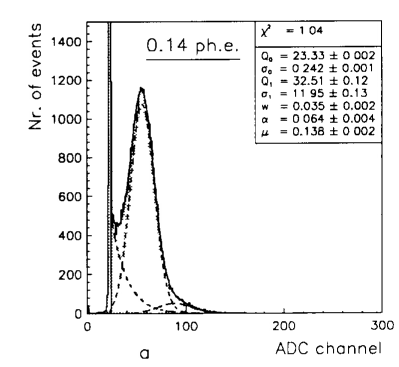
\includegraphics[height=7cm]{images/spe_sreal.png}
    \caption{单光子模式下的电荷谱}
    \label{fig:spe_sreal}
\end{figure}

但在JUNO光电倍增管测试中,发现MCP-PMT电荷谱存在长尾巴\cite{2021Gain}:
\begin{figure}[ht]
    \centering
    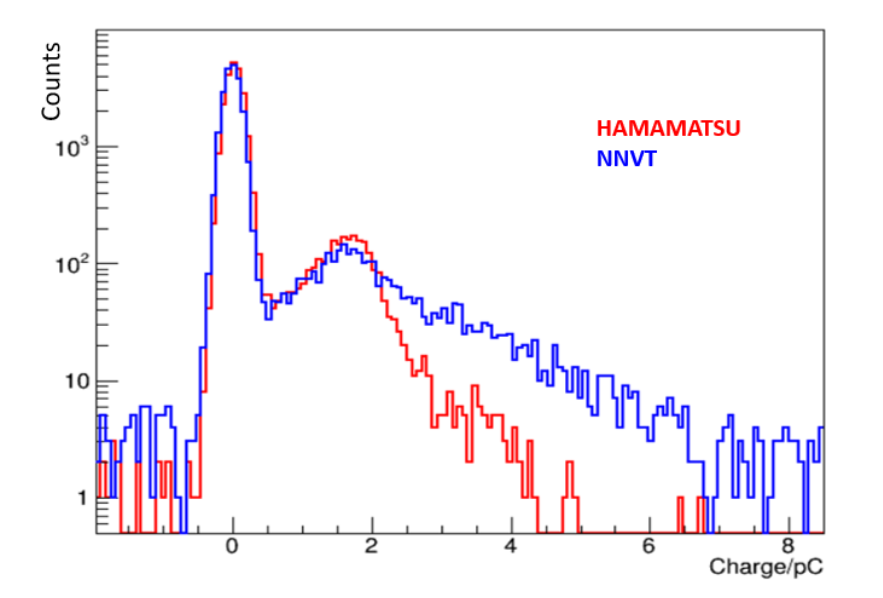
\includegraphics[height=6cm]{images/JUNO_spe.png}
    \caption{JUNO测试PMT中,20-inch MCP-PMT单光电子响应(蓝色),20-inch dynode PMT单光电子响应(红色)}
    \label{fig:spe_JUNO}
\end{figure}

考虑到MCP表面镀有二次发射材料,因此,入射到MCP表面的电子存在产生多个二次电子或弹性散射电子进入到MCP孔洞中进行倍增,产生多高斯峰的叠加,形成长尾巴结构。但电子入射到MCP表面产生的二次电子能量存在一定的分布,因此需要对不同入射能量的电子进行增益的刻度\cite{2020Analysis}:
\begin{figure}[ht]
    \centering
    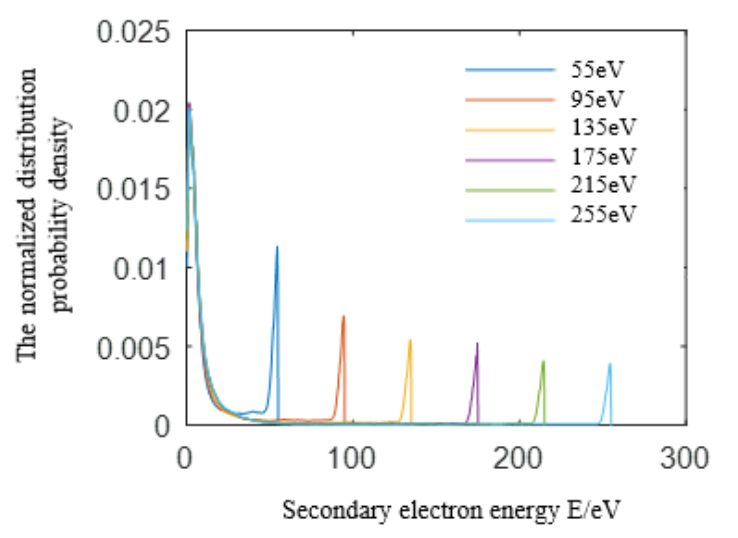
\includegraphics[height=7cm]{images/sey.png}
    \caption{电子入射到二次发射材料表面,产生不同能量的二次电子能量分布。}
    \label{fig:sey}
\end{figure}

\section{实验设计与期望}
通过入射不同能量的电子到达MCP表面,保持MCP的增益为1.0$\times 10^7$,测量不同能量电子的增益,
并通过加反向电压的方式,将直接入射进入MCP孔中电子与MCP表面产生二次电子(包括弹性散射电子)的渡越时间分开,通过不同的渡越时间,将二次电子与直入射电子区别开来。
\subsection{实验电路}
8-inch光电倍增管分压如图  \ref{fig:el}:
\begin{figure}[ht]
    \centering
    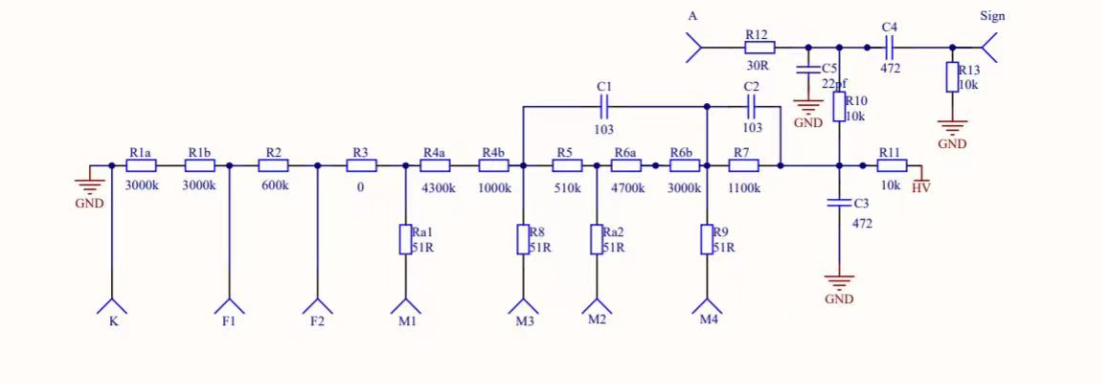
\includegraphics[height=4cm]{images/el.png}
    \caption{MCP-PMT的分压示意图,$K$与$F_1$之间为光阴极到聚焦极间的电压,$F_1$与$F_2$之间为聚焦极到MCP表面的电压,$M_1$与$HV$之间为MCP的倍增电压。}
    \label{fig:el}
\end{figure}
简化后电路可分为三部分:光阴极到聚焦极的电压($R_{K-F_1}$),聚焦极到MCP表面的电压($R_{F_1-F_2}$),以及MCP的倍增电压($R_{M_1-HV}$) :。通过保持MCP的倍增电压不变,可以保持MCP的倍增增益不变。假设光阴极在单光子模式下产生的电子能量比较低,大概在几个$eV$量级,则入射到MCP表面的电子能量主要由光阴极到聚焦极的电压与聚焦极到MCP表面的电压所决定,则可以通过调整该部分的电阻来调整电压分布,调整电子入射到MCP表面的能量。将MCP-PMT工作在1.0$\times 10^7$增益下,可得到其工作电压,记为$V_0$,则可以通过电阻关系,得到MCP所分电压为:
\begin{equation}
    V_{MCP}=V_0\times \frac{R_{M_1-HV}}{R_{M_1-HV}+R_{K-F_1}+R_{F_1-F_2}}
\end{equation}
现将电路改造如下,将$F_1$转接到$M_2$处,如图 \ref{fig:elg}:
\begin{figure}[ht]
    \centering
    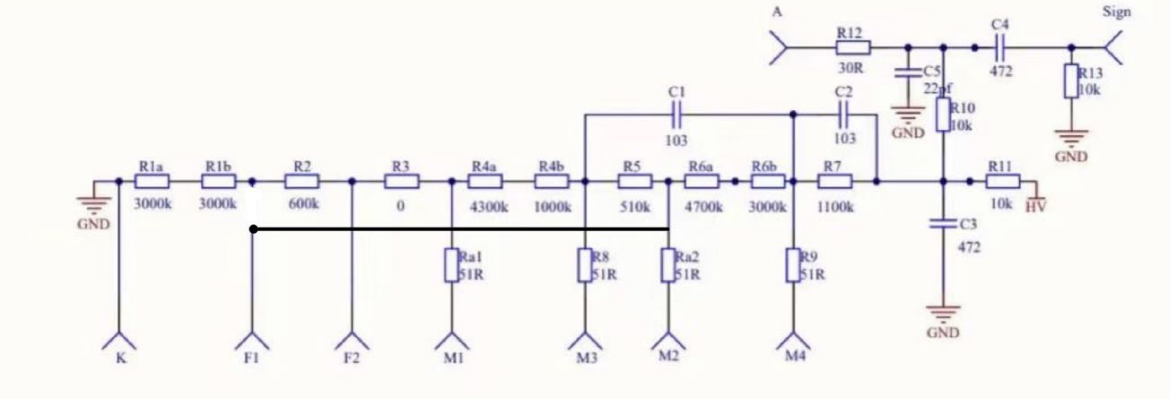
\includegraphics[height=4cm]{images/elg.png}
    \caption{将$F_1$转接到$M_2$,改为将聚焦极到MCP的聚焦电压改为反向电压。}
    \label{fig:elg}
\end{figure}
此时,可以通过调整如图 \ref{fig:elg}中的$R_{1a},R_{1b}$与$R_2$,调整入射到MCP表面的电子的能量,且保持MCP倍增电压不变的情况下,入射到MCP表面的电子能量大小为:
\begin{equation}
    V = V_0\times \frac{R_{1a}+R_{1b}+R_2}{R_{M_1-HV}+R_{K-F_1}+R_{F_1-F_2}}
\end{equation}
现使用的MCP-PMT为PM2104-9085,$V_0=1792V$,在不改变分压电路时,阻值与图\ref{fig:el}中一致,$R_{M_1-HV}=14620k\Omega,\ R_{K-F_1}=6000k\Omega,\ R_{F_1-F_2}=600k\Omega$。

通过测量不同能量的电子入射到MCP中所得的电荷增益,期望得到如图 \ref{fig:gain}的曲线,与二次发射电子的能谱如图 \ref{fig:sey}卷积,期望得到MCP的长尾巴机制。
\begin{figure}[ht]
    \centering
    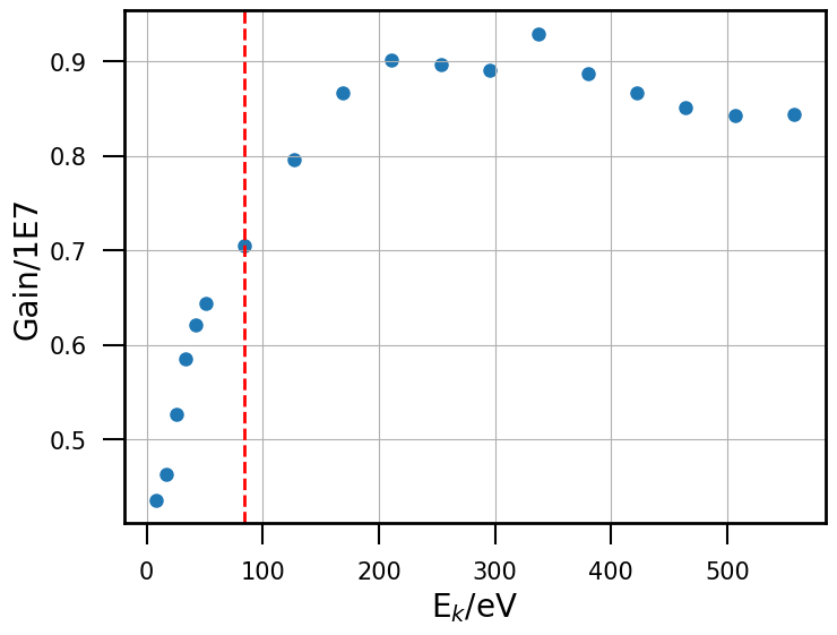
\includegraphics[height=6cm]{images/gain.png}
    \caption{不同能量的电子在MCP中的增益曲线。}
    \label{fig:gain}
\end{figure}

同时,入射到MCP表面的电子是否会产生二次电子或者弹性散射电子,或着说这个过程发生的概率多大,关系到卷积获得电荷增益谱时的比例。如果能通过反向电压的延时将单个高能量电子和多个低能量电子事例区分开来,则能获得准确的发生二次发射和弹性散射的比例。因此,我们期望所加的反向电压有足够的延时效应。

\subsection{MCP增益稳定}
在测试MCP增益随电子能量变化的过程中,应保持MCP孔中的增益稳定,本实验方案中通过控制梯度电压稳定的方案实现,在实际数据中,采集到的相同大小的电荷的波形应保持一致。
\subsection{聚焦电压的作用}
\subsection{模拟研究}
从图\ref{fig:sey}中可以看出,无论电子能量多大,产生的二次发射电子能量主要集中在低能量,也就是100$eV$以内,因此,需要通过模拟来衡量从MCP表面产生的电子再返回到MCP表面的时间;电子的发射是随机的,通过不同的角度发射,获取大致的二次电子的延时时间。如果在分析时能获得准确的电荷时间谱,也就是渡越时间,可以通过模拟指导的延迟时间处的事例比例,大致给出产生低能量二次发射电子的比例和产生弹性散射电子的比例,在卷积不同电子能量增益和二次电子能谱以获得MCP-PMT增益时,能提供参考和验证。
\section{FSMP波形分析}
将FSMP波形分析方法应用到MCP-PMT测试中,期望得到准确的电荷和渡越时间,以实现上述的想法。
目前遇到的困难主要是代码难以读懂,可以参考的过程文件太少。
test部分的使用。

\newpage

\section{论文汇:PMT统计学模型}
如果一个统计学事件,类似于一个初级电子发射多个二次电子,$s=0,1,2...$,且其概率为$p_0,p_1,p_2...$,则借助辅助变量$x$将其产生函数写为:
\begin{equation}
    G(x)=\sum_s p_s x^s
\end{equation}
具有以下性质:
\begin{enumerate}
    \item {$G(1)=1$}
    \item {$\bar{s}=G^{\prime}(1)$}
    \item {$\sigma^2=\bar{s^2}-\bar{s}^2=G^{\prime\prime}(1)+G^{\prime}(1)-[G^{\prime}(1)]^2$}
\end{enumerate}
光电倍增管将一个电子经过多次放大后形成电信号,这其中可以看作是多个电极之间放大的级联事件。考虑事件$A,B$,对应的生成函数为$A(x),B(x)$,则二者的级联事件$G$的生成函数为:$G(x)=A[B(x)]$,则有以下性质:
\begin{enumerate}
    \item {$\bar{s}=G^{\prime}(1)=G^{\prime}(B(1))\times B^{\prime}(1)=\bar{s_A}\bar{s_B}$}
    \item {$\sigma^2=\bar{s^2}-\bar{s}^2=G^{\prime\prime}(1)+G^{\prime}(1)-[G^{\prime}(1)]^2=\bar{s_B}^2\sigma_A^2+\bar{s_A}\sigma_B^2$}
\end{enumerate}

定义相对方差:$\mathscr{V}= \frac{\sigma^2}{\bar{s}^2}$,则有:
\begin{equation}
    \mathscr{V}=\mathscr{V}_A+\frac{\mathscr{V}_B}{\bar{s}_A}
\end{equation}

推广到多个变量:
\begin{equation}
    \begin{gathered}
        \bar{s}=\bar{s}_1 \bar{s}_2 \ldots \bar{s}_n \\
        \mathscr{V}=\mathscr{V}{ }_1+\frac{\mathscr{V}_2}{\bar{s}_1}+\ldots+\frac{\mathscr{V_{ n }}}{\bar{s}_1 \bar{s}_2 \ldots \bar{s}_{n-1}}
    \end{gathered}
\end{equation}

在光电倍增管中,假设第$n$级的放大增益为$m_n$,则整个管子的放大的增益可以写为:
\begin{equation}
    \bar{G}=\bar{m}_1 \bar{m}_2 \ldots \bar{m}_n
\end{equation}

相对方差为:
\begin{equation}
    \mathscr{V}_G=\mathscr{V}{ }_1+\frac{\mathscr{V}_2}{\bar{m}_1}+\ldots+\frac{\mathscr{V_{ n }}}{\bar{m}_1 \bar{m}_2 \ldots \bar{m}_{n-1}}
\end{equation}

假设每一级的放大是相同,具有相同的均值和方差,则有:
\begin{equation}
    \mathscr{V}_G=\mathscr{V}\frac{\bar{m}^n-1}{(\bar{m}-1)\bar{m}^{n-1}}
\end{equation}
在$\bar{m}^n\gg 1$时,有$\mathscr{V}_G=\mathscr{V}\frac{\bar{m}}{\bar{m}-1}$,由此,相对方差并不依赖于放大的级数,而主要依赖于每一级放大的相对方差。

实际上,为了提高第一级的收集效率,第一级的聚焦电压往往更高,在这种情况下:
\begin{equation}
    \mathscr{V}_G=\mathscr{V}_1+\mathscr{V} \frac{\bar{m}}{\bar{m}_1(\bar{m}-1)}
\end{equation}
\section{MCP-PMT的统计学模型}
实际上,对于MCP-PMT而言,我们可以将光电子到达MCP上表面之后的倍增过程分为两种类型:
\begin{enumerate}
    \item {光电子直接进入到MCP孔中倍增}
    \item {光电子在MCP表面二次发射,形成的二次发射电子进入到MCP中倍增}
\end{enumerate}
对于第二种情况,可以将PMT的倍增过程分解为,在MCP表面的“第一次倍增”,之后进入到孔种的倍增过程则是为第二次倍增,只不过由于在孔中的电子能量比较小,第二次的倍增显得没有那么充分,之后的第三次、第四次倍增则和直接入射的倍增过程应该是基本相同的;之前的实验已经说明,低能量的电子入射到MCP孔中,形成的增益信号是比较小的,通常会显著的小于1个正常的PE大小,但对于这种情况而言,进入到MCP中的电子往往不只是一个,所以最终在电荷谱上形成的信号看起来是并不小。

因此,可以使用双高斯的函数来对单光子模式下的MCP-PMT电荷相应进行建模:
\begin{equation}
    charge = A_{sig}N(x;\mu_{sig},\sigma_{sig})+A_{MCP}N(x;\mu_{MCP},\sigma_{MCP})
\end{equation}
其中,sig部分描述的是直接进入到MCP孔中的光电子的电荷相应,MCP部分为打在MCP表面的光电子的电荷相应。在这种模型下,我们并不需要知道长尾巴是由多少个MCP电子形成的,相比之下,第二种模型发射的概率是我们更关心的。


\bibliographystyle{plain}
\bibliography{ref}
\end{document}


